\section{Ergebnisse Usability Test}
\textcolor{blue}{\textit{einleitende Worte}}\\

\subsection{Fehlerbetrachtung}
- Fehlende Daten

\subsection{...}
\begin{table}[H]
\begin{tabular}{|l|c|c|c|c|}
\hline
Aufgabe 1   & $\Bar{x}$ & $\Tilde{x}$ & $\sigma$ & f \\ \hline
alt         & xxxx      &  xx         &  xxxx &  xxx   \\ \hline
neu         & xxxx      &  xx         &  xxxx &  xxx   \\ \hline
Differenz   &           &             & -     &  xxx   \\ \hline
\end{tabular}
\begin{tabular}{|l|c|c|c|c|}
\hline
Aufgabe 2   & $\Bar{x}$ & $\Tilde{x}$ & $\sigma$ & f \\ \hline
alt         & xxxx      &  xx         &  xxxx &  xxx   \\ \hline
neu         & xxxx      &  xx         &  xxxx &  xxx   \\ \hline
Differenz   &           &             & -     &  xxx   \\ \hline
\end{tabular}
\begin{tabular}{|l|c|c|c|c|}
\hline
Aufgabe 3.1   & $\Bar{x}$ & $\Tilde{x}$ & $\sigma$ & f \\ \hline
alt         & xxxx      &  xx         &  xxxx &  xxx   \\ \hline
neu         & xxxx      &  xx         &  xxxx &  xxx   \\ \hline
Differenz   &           &             & -     &  xxx   \\ \hline
\end{tabular}
\begin{tabular}{|l|c|c|c|c|}
\hline
Aufgabe 3.2   & $\Bar{x}$ & $\Tilde{x}$ & $\sigma$ & f \\ \hline
alt         & xxxx      &  xx         &  xxxx &  xxx   \\ \hline
neu         & xxxx      &  xx         &  xxxx &  xxx   \\ \hline
Differenz   &           &             & -     &  xxx   \\ \hline
\end{tabular}
\begin{tabular}{|l|c|c|c|c|}
\hline
Aufgabe 4.1   & $\Bar{x}$ & $\Tilde{x}$ & $\sigma$ & f \\ \hline
alt         & xxxx      &  xx         &  xxxx &  xxx   \\ \hline
neu         & xxxx      &  xx         &  xxxx &  xxx   \\ \hline
Differenz   &           &             & -     &  xxx   \\ \hline
\end{tabular}
\begin{tabular}{|l|c|c|c|c|}
\hline
Aufgabe 4.2   & $\Bar{x}$ & $\Tilde{x}$ & $\sigma$ & f \\ \hline
alt         & xxxx      &  xx         &  xxxx &  xxx   \\ \hline
neu         & xxxx      &  xx         &  xxxx &  xxx   \\ \hline
Differenz   &           &             & -     &  xxx   \\ \hline
\end{tabular}
\begin{tabular}{ll}
\multicolumn{2}{l}{verwendete Formelzeichen:} \\ \hline
$\Bar{x}$          & Mittelwert               \\
$\Tilde{x}$        & Median                   \\
$\sigma$           & Standardabweichung       \\
f                  & Fehlerquote
\end{tabular}
\caption{Zusammenfassung der Ergebnisse des Usability-Tests}
\label{tab:usability_tabellen}
\end{table}
% \autoref{tab:usability_tabellen}

\subsection{Zeitvergleich}
- t-Test Beispielrechnung (einseitig, gepaart)\\
- Tabelle mit t-Test-Ergebnissen\\
-> verweisen auf Ergebnisse aus Excel: $=TTEST(Matrix_{alt}, Matrix_{neu},1,1)$\\
-> erster t-Test zum Verständnis\\
-> erst Normalverteiltes Ergebnis\cite{normalverteilung_rechner}

\subsection{Genauigkeit-Zeit}
\begin{figure}[H]
    \centering
    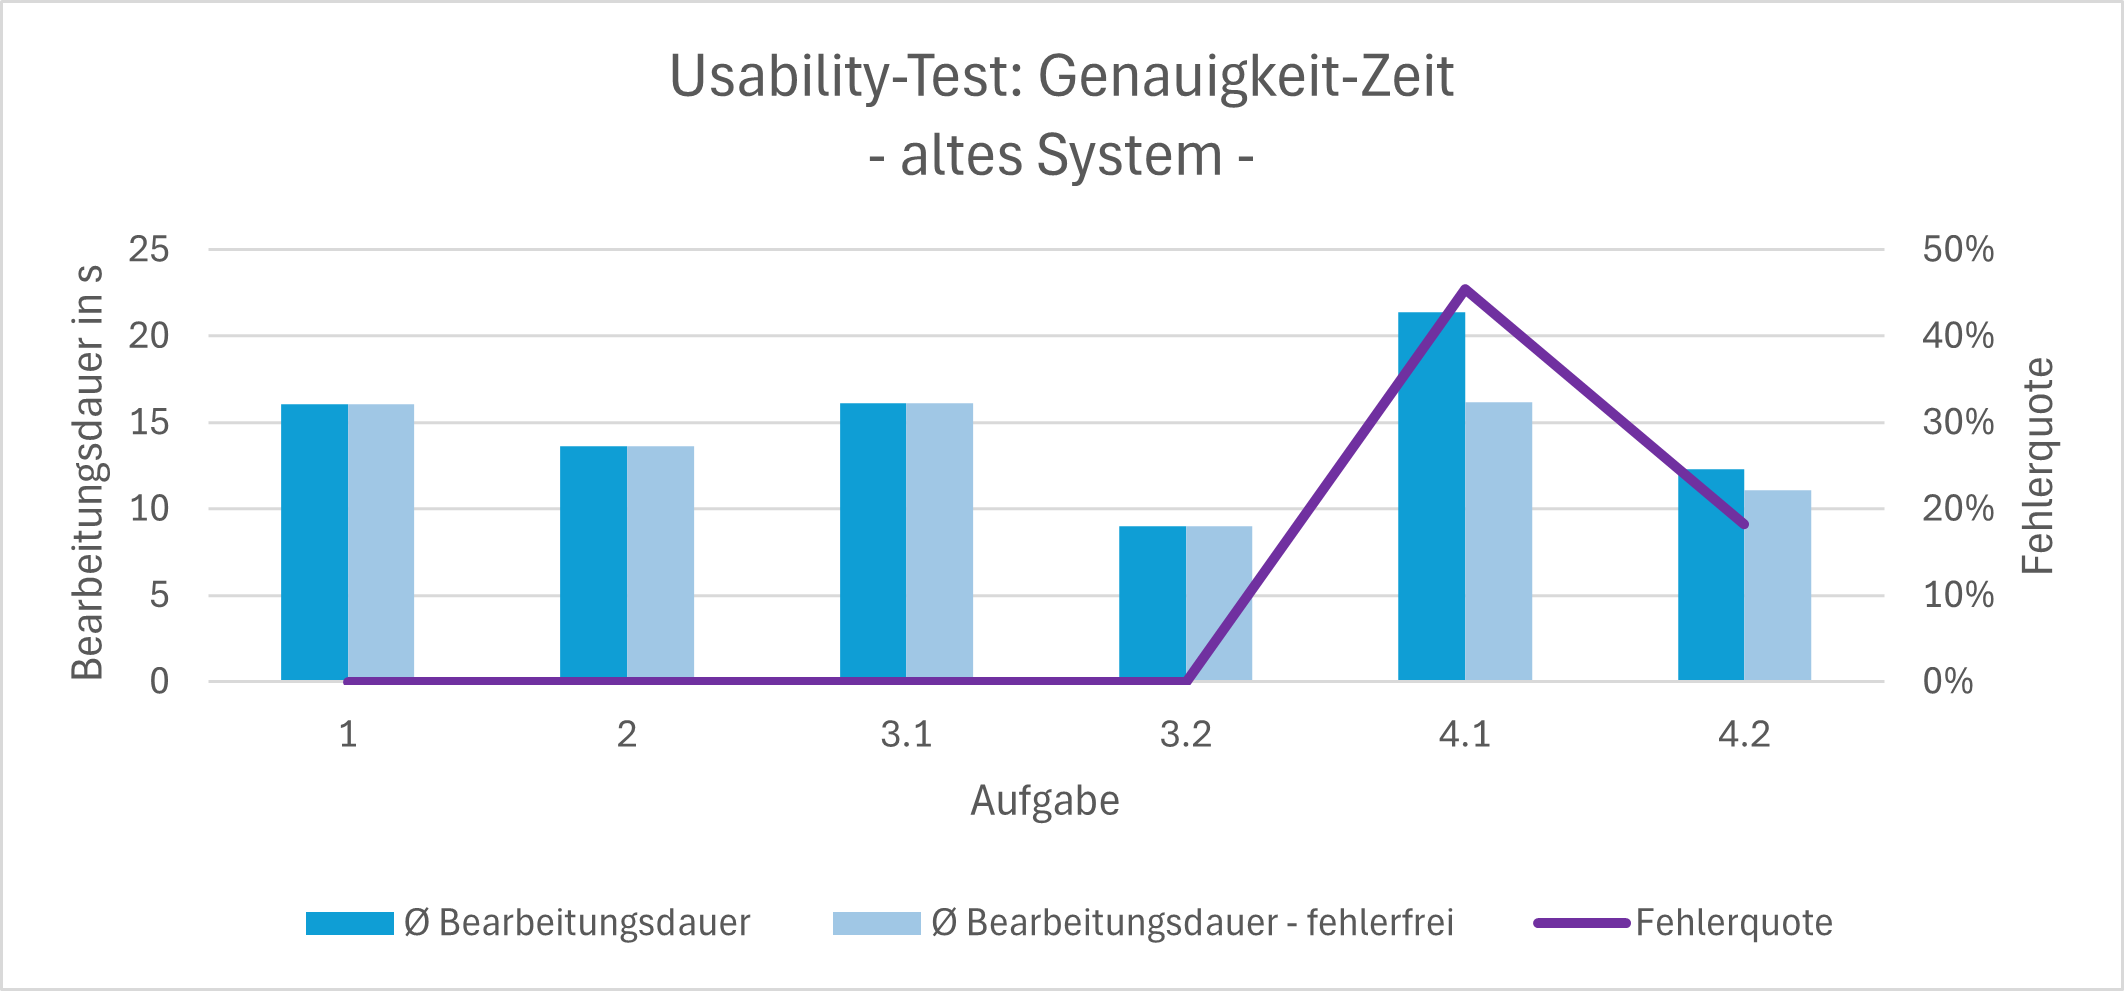
\includegraphics[width=0.8\linewidth]{Diagramme/usability_genauigkeit-zeit_alt.png}
    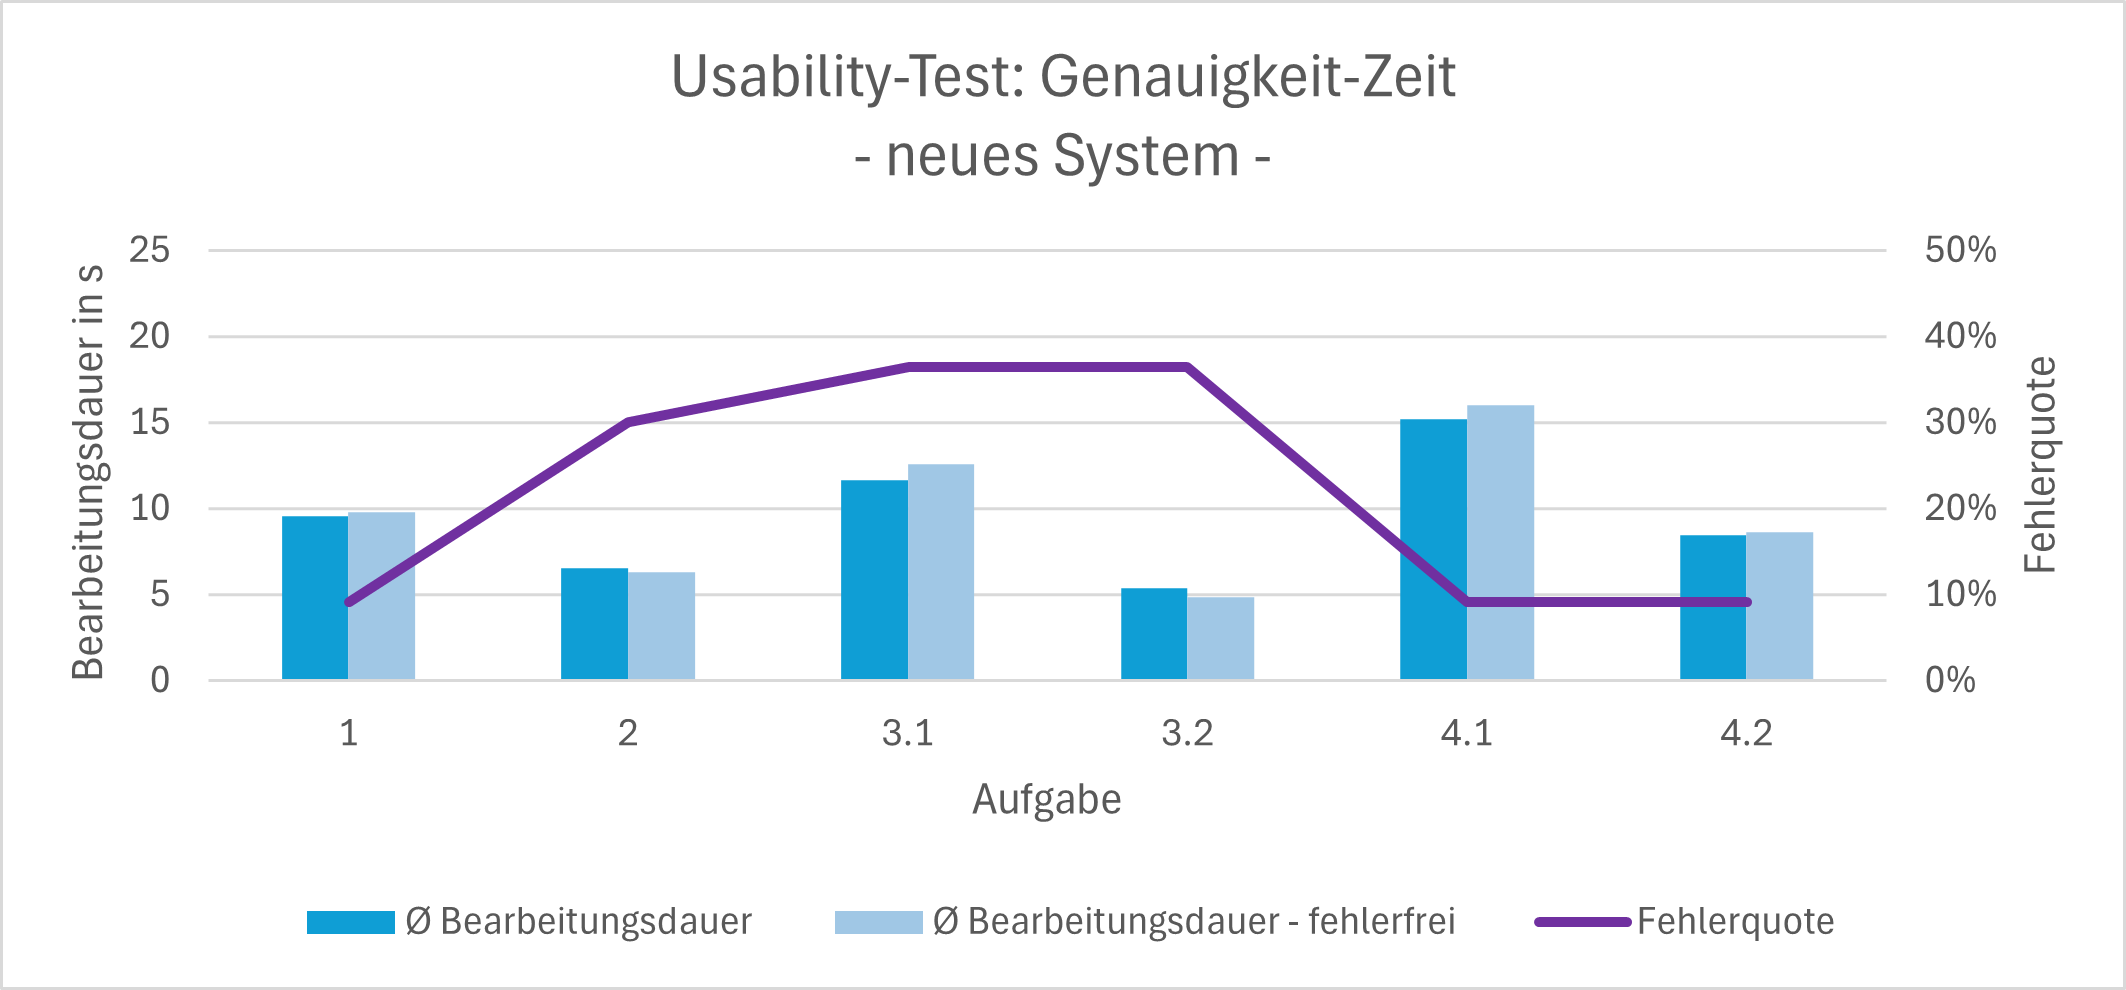
\includegraphics[width=0.8\linewidth]{Diagramme/usability_genauigkeit-zeit_neu.png}
    \caption{Usability-Test: Vergleich Genauigkeit-Zeit im alten und neuen System}
    \label{fig:usability_genauigkeit-zeit_alt-neu}
\end{figure}
\begin{figure}[H]
    \centering
    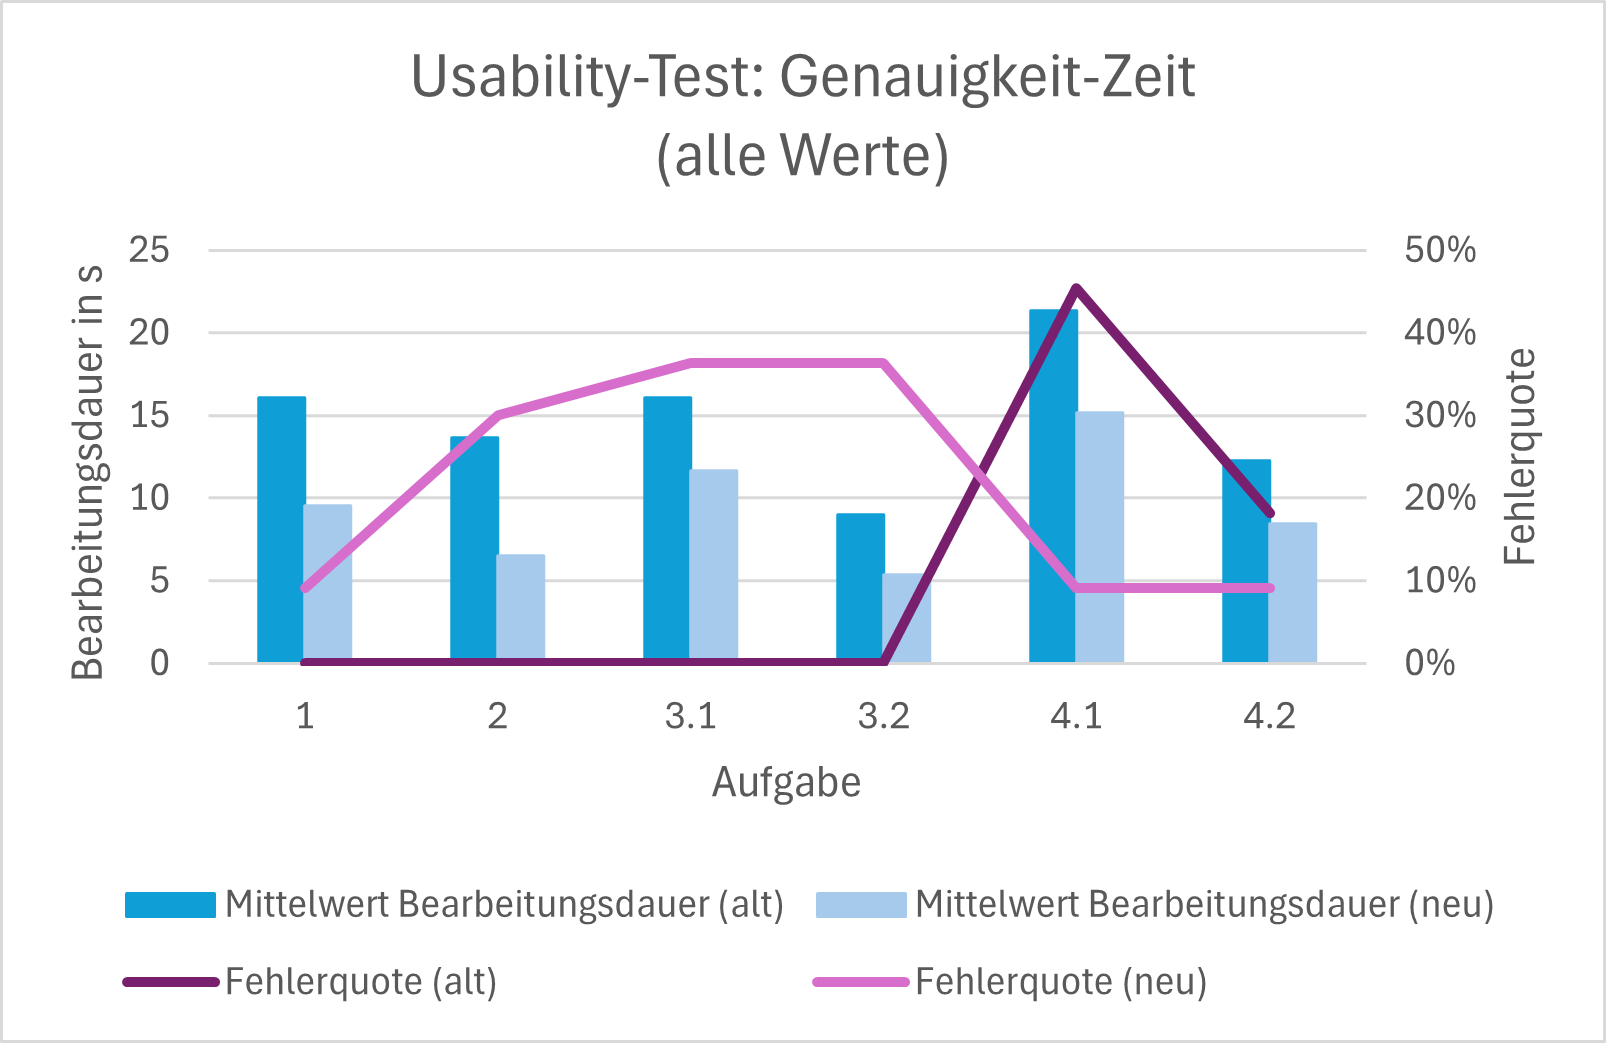
\includegraphics[width=0.8\linewidth]{Diagramme/usability_genauigkeit-zeit_alle.png}
    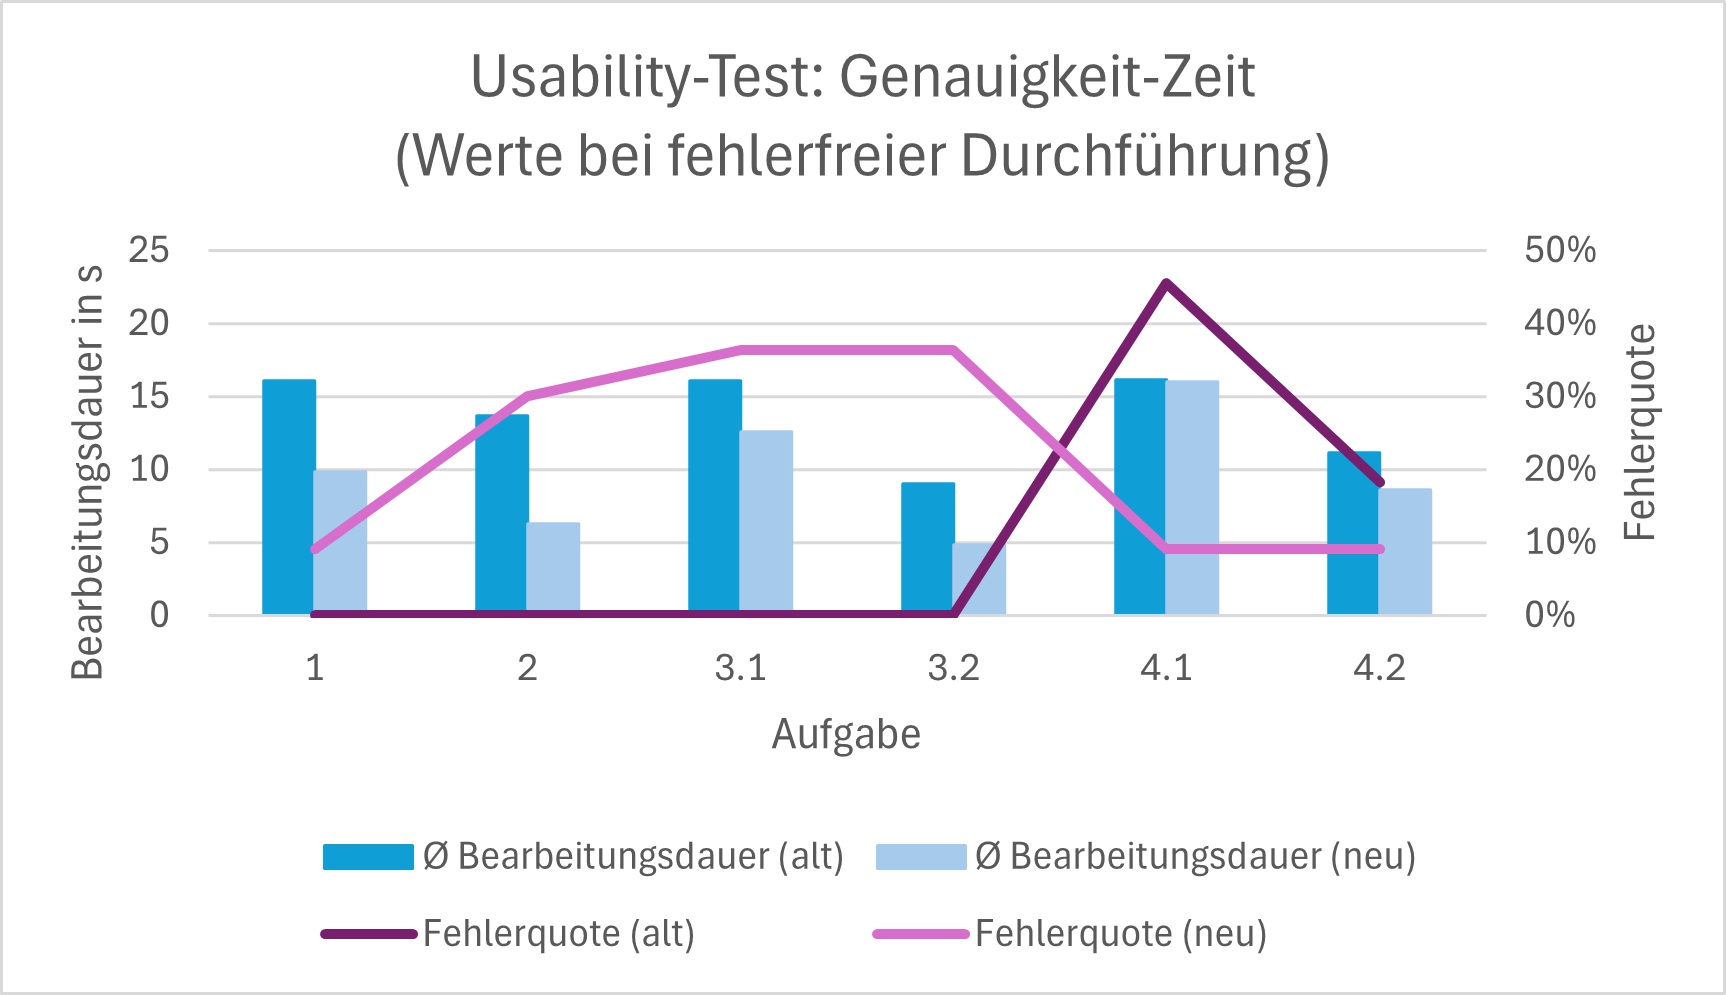
\includegraphics[width=0.8\linewidth]{Diagramme/usability_genauigkeit-zeit_richtige.png}
    \caption{Usability-Test: Zeitvergleich von allen Werten und nur richtigen Antworten - im Verhältnis zur Fehlerquote}
    \label{fig:usability_genauigkeit-zeit_alle-richtige}
\end{figure}
- neu ist in jeder Aufgabe schneller
- Fehlerquote nicht überall eindeutig

\begin{figure}[H]
    \centering
    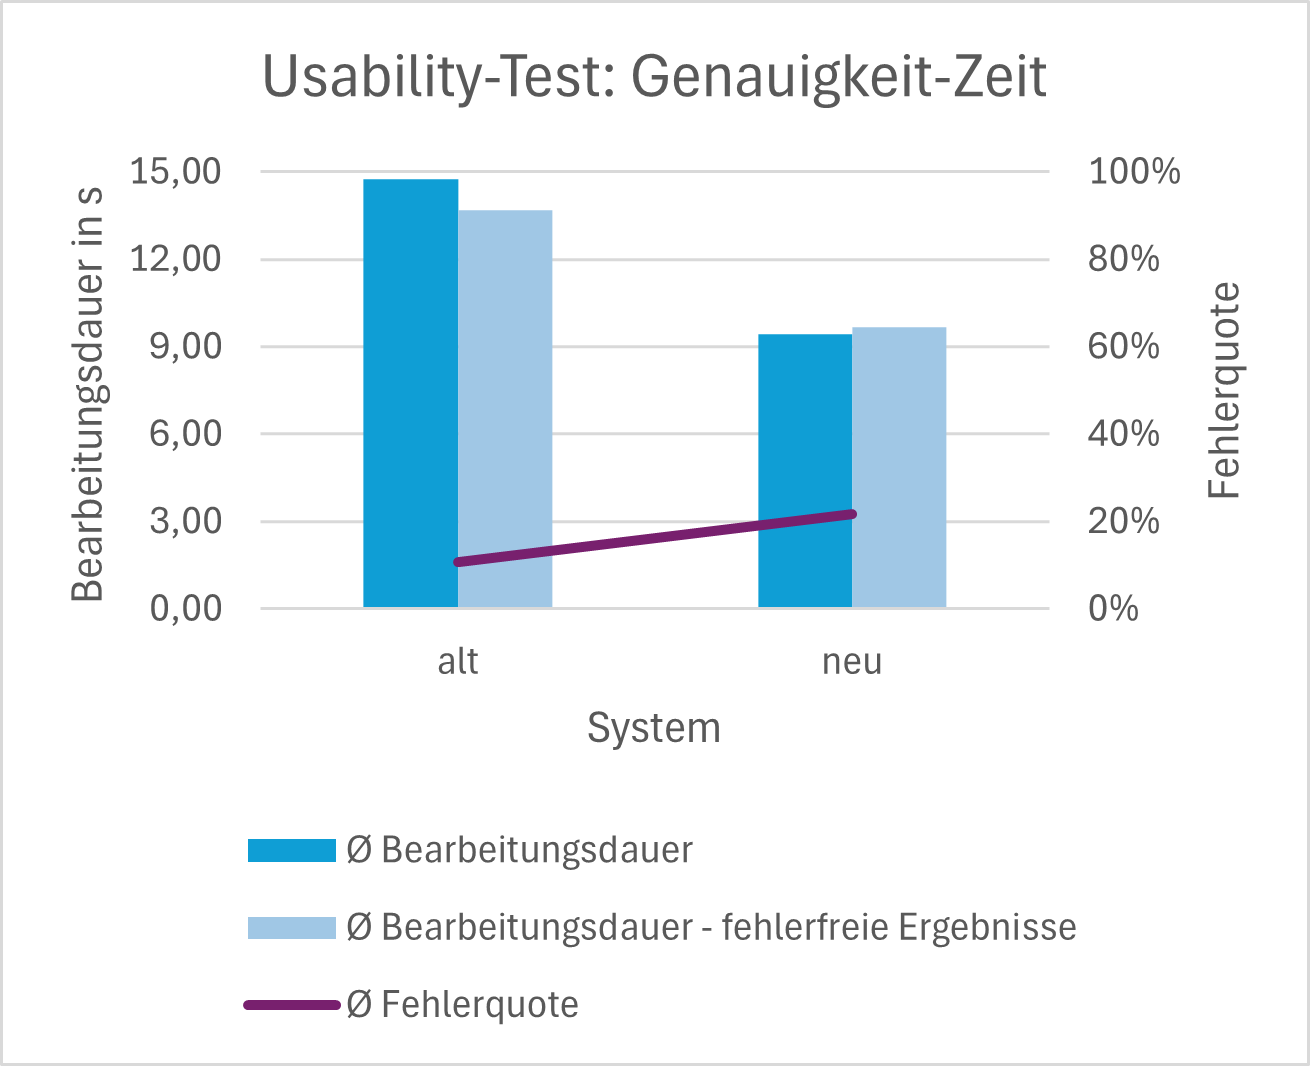
\includegraphics[width=0.8\linewidth]{Diagramme/usability_genauigkeit-zeit_mittel.png}
    \caption{Usability-Test: Vergleich der mittleren Bearbeitungsdauer - im Verhältnis zur Fehlerquote}
    \label{fig:usability_genauigkeit-zeit_mittel}
\end{figure}
- neu ist im Mittel schneller\\
- aber auch Fehlerquote bei neu im MIttel höher

